%---------------------------------------------------------------------
\section{O m�todo MRAC indireto}

O m�todo MRAC indireto consiste em uma realimentac�o de sa�da utilizando um ganho variante no tempo, que � estimado atrav�s da adaptac�o do p�lo incerto da planta, como � evidente de acordo com \eqref{eq:ctrl_law} e \eqref{eq:est_gain}. 

\begin{figure}[H]
  \centering
  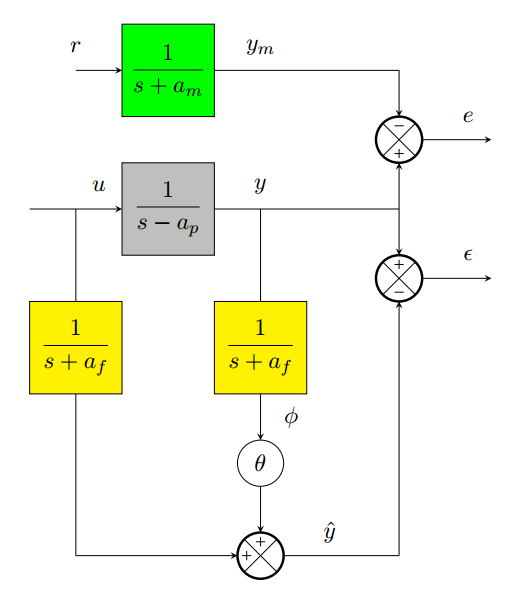
\includegraphics[scale=0.6]{figs/blocks/estruturaMRAC_indireto.png}
  \caption{Estrutura do MRAC indireto.}
\end{figure}

Como em outros esquemas MRAC, este controle possui um modelo de refer�ncia
desejado que � utilizado para a gera��o de um sinal de erro de sa�da \eqref{eq:error}. Ele tamb�m possui um filtro est�vel de primeira ordem que � aplicado sobre os sinais de entrada e sa�da. Assim, � poss�vel escrever a sa�da do sistema como
%
\begin{equation}
y = \theta^* \, \phi + \mathcal{L}^{-1}\left\{ \frac{u}{s+a_f} \right\} \,,
\quad \theta^* = a_f + a_p \,,
\label{eq:saida}
\end{equation}
%
motivando portanto a \textit{defini��o} da predi��o de sa�da dada por \eqref{eq:pred_saida}. Assim, utilizando \eqref{eq:pred_error}, \eqref{eq:pred_saida} e \eqref{eq:saida} temos:
%
\begin{flalign}
\epsilon &= \hat{y} - y \nonumber \\
&= \theta \, \phi + \mathcal{L}^{-1}\left\{ \frac{U}{s+a_f} \right\} - \theta^*
\, \phi - \mathcal{L}^{-1}\left\{ \frac{U}{s+a_f} \right\} \nonumber \\
&= ( \theta - \theta^*) \, \phi = \tilde{\theta} \, \phi \,.
\label{eq:pred_error2}
\end{flalign}

Utilizando a candidata � fun��o de Lyapunov $2V(\tilde{\theta}) = \gamma^{-1} \, \tilde{\theta}^2$, derivando no tempo e aplicando a lei de adapta��o \eqref{eq:adpt_law}, obtemos:
%
$$\dot{V} = -\frac{\epsilon^2}{m^2} \leq 0 \,.$$
%
Portanto, conclui-se que $\tilde{\theta} \in \mathcal{L}_{\infty}$ e ainda:
%
$$ \int^{\infty}_{0} \frac{\epsilon^2}{m^2} \le \infty \,, \int^{\infty}_{0} \dot{\theta}^2 \le \infty \,.$$
%
Utilizando estes resultados, � poss�vel demonstrar que $\epsilon \rightarrow 0,
e_0 \rightarrow 0$.

Alternativamente, podemos usar a parametriza��o $\theta^* = a_p$, e, em vez da
Equa��o \eqref{eq:saida}, obtemos uma equa��o similar para a sa�da $y$
\eqref{eq:saida2}:
 \begin{equation}
y - \mathcal{L}^{-1}\left\{ \frac{a_fY}{s+a_f} \right\}= \theta^* \, \phi +
\mathcal{L}^{-1}\left\{ \frac{U}{s+a_f} \right\} \,, \quad \theta^* = a_p \,,
\label{eq:saida2}
\end{equation}